\documentclass[10pt,journal]{IEEEtran}
\usepackage[letterpaper,top=1in,bottom=1in,left=.7in,right=.7in,columnsep=.2in]{geometry}
\usepackage{amsmath,amssymb,graphicx,booktabs,array,fontspec,balance}
\usepackage[hidelinks]{hyperref}
\setmainfont{Times New Roman}
\newtheorem{proposition}{Proposition}
\newtheorem{corollary}{Corollary}
\newcommand{\norm}[1]{\lVert#1\rVert}
\newcommand{\R}{\mathbb R}
\newcommand{\um}{\,\mu\mathrm{rad}}
\newcommand{\NPrimary}{10,800}
\newcommand{\NSensitivity}{18,450}
\newcommand{\NTotal}{29,250}
\newcommand{\UADDriftOutage}{4.9730}
\newcommand{\UADDriftAccepted}{93}
\newcommand{\UADDriftEnergy}{7.030}
\newcommand{\UADDriftPninetyfive}{12.000}
\newcommand{\UADDriftAbstained}{6}
\newcommand{\UADDriftError}{0.291}
\newcommand{\DAPDriftOutage}{4.2462}
\newcommand{\DAPDriftAccepted}{100}
\newcommand{\DAPDriftEnergy}{28.725}
\newcommand{\DAPDriftPninetyfive}{4.480}
\newcommand{\DAPDriftAbstained}{0}
\newcommand{\DAPDriftError}{0.130}
\newcommand{\FixedDriftOutage}{4.2226}
\newcommand{\FixedDriftAccepted}{100}
\newcommand{\FixedDriftEnergy}{63.981}
\newcommand{\FixedDriftPninetyfive}{4.540}
\newcommand{\FixedDriftAbstained}{0}
\newcommand{\FixedDriftError}{0.115}
\newcommand{\KFDriftOutage}{4.2226}
\newcommand{\KFDriftAccepted}{100}
\newcommand{\KFDriftEnergy}{63.981}
\newcommand{\KFDriftPninetyfive}{4.540}
\newcommand{\KFDriftAbstained}{0}
\newcommand{\KFDriftError}{0.122}
\newcommand{\ESDriftOutage}{4.2658}
\newcommand{\ESDriftAccepted}{0}
\newcommand{\ESDriftEnergy}{1719.690}
\newcommand{\ESDriftPninetyfive}{5.362}
\newcommand{\ESDriftAbstained}{0}
\newcommand{\ESDriftError}{nan}
\newcommand{\UADPointingOutage}{3.5980}
\newcommand{\UADPointingAccepted}{93}
\newcommand{\UADPointingEnergy}{7.030}
\newcommand{\UADPointingPninetyfive}{12.000}
\newcommand{\UADPointingAbstained}{6}
\newcommand{\UADPointingError}{0.291}
\newcommand{\DAPPointingOutage}{2.7338}
\newcommand{\DAPPointingAccepted}{100}
\newcommand{\DAPPointingEnergy}{28.725}
\newcommand{\DAPPointingPninetyfive}{3.100}
\newcommand{\DAPPointingAbstained}{0}
\newcommand{\DAPPointingError}{0.130}
\newcommand{\FixedPointingOutage}{2.7342}
\newcommand{\FixedPointingAccepted}{100}
\newcommand{\FixedPointingEnergy}{63.981}
\newcommand{\FixedPointingPninetyfive}{3.160}
\newcommand{\FixedPointingAbstained}{0}
\newcommand{\FixedPointingError}{0.115}
\newcommand{\KFPointingOutage}{2.7342}
\newcommand{\KFPointingAccepted}{100}
\newcommand{\KFPointingEnergy}{63.981}
\newcommand{\KFPointingPninetyfive}{3.160}
\newcommand{\KFPointingAbstained}{0}
\newcommand{\KFPointingError}{0.123}
\newcommand{\ESPointingOutage}{2.4426}
\newcommand{\ESPointingAccepted}{0}
\newcommand{\ESPointingEnergy}{1646.500}
\newcommand{\ESPointingPninetyfive}{3.300}
\newcommand{\ESPointingAbstained}{0}
\newcommand{\ESPointingError}{nan}
\newcommand{\UADNearOutage}{0.0000}
\newcommand{\UADNearAccepted}{0}
\newcommand{\UADNearEnergy}{0.000}
\newcommand{\UADNearPninetyfive}{0.000}
\newcommand{\UADNearAbstained}{100}
\newcommand{\UADNearError}{nan}
\newcommand{\DAPNearOutage}{0.0000}
\newcommand{\DAPNearAccepted}{0}
\newcommand{\DAPNearEnergy}{0.000}
\newcommand{\DAPNearPninetyfive}{0.000}
\newcommand{\DAPNearAbstained}{100}
\newcommand{\DAPNearError}{nan}
\newcommand{\FixedNearOutage}{2.2826}
\newcommand{\FixedNearAccepted}{100}
\newcommand{\FixedNearEnergy}{63.981}
\newcommand{\FixedNearPninetyfive}{2.300}
\newcommand{\FixedNearAbstained}{0}
\newcommand{\FixedNearError}{0.050}
\newcommand{\KFNearOutage}{2.2826}
\newcommand{\KFNearAccepted}{100}
\newcommand{\KFNearEnergy}{63.981}
\newcommand{\KFNearPninetyfive}{2.300}
\newcommand{\KFNearAbstained}{0}
\newcommand{\KFNearError}{0.047}
\newcommand{\ESNearOutage}{4.6764}
\newcommand{\ESNearAccepted}{0}
\newcommand{\ESNearEnergy}{138.376}
\newcommand{\ESNearPninetyfive}{4.820}
\newcommand{\ESNearAbstained}{0}
\newcommand{\ESNearError}{nan}
\newcommand{\UADFadingOutage}{11.8744}
\newcommand{\UADFadingAccepted}{0}
\newcommand{\UADFadingEnergy}{6.880}
\newcommand{\UADFadingPninetyfive}{12.000}
\newcommand{\UADFadingAbstained}{8}
\newcommand{\UADFadingError}{nan}
\newcommand{\DAPFadingOutage}{11.7712}
\newcommand{\DAPFadingAccepted}{0}
\newcommand{\DAPFadingEnergy}{27.863}
\newcommand{\DAPFadingPninetyfive}{12.000}
\newcommand{\DAPFadingAbstained}{3}
\newcommand{\DAPFadingError}{nan}
\newcommand{\FixedFadingOutage}{11.6960}
\newcommand{\FixedFadingAccepted}{0}
\newcommand{\FixedFadingEnergy}{63.981}
\newcommand{\FixedFadingPninetyfive}{12.000}
\newcommand{\FixedFadingAbstained}{0}
\newcommand{\FixedFadingError}{nan}
\newcommand{\KFFadingOutage}{2.8116}
\newcommand{\KFFadingAccepted}{100}
\newcommand{\KFFadingEnergy}{63.981}
\newcommand{\KFFadingPninetyfive}{3.180}
\newcommand{\KFFadingAbstained}{0}
\newcommand{\KFFadingError}{0.904}
\newcommand{\ESFadingOutage}{2.4452}
\newcommand{\ESFadingAccepted}{0}
\newcommand{\ESFadingEnergy}{1819.610}
\newcommand{\ESFadingPninetyfive}{3.300}
\newcommand{\ESFadingAbstained}{0}
\newcommand{\ESFadingError}{nan}
\newcommand{\UADNoisyDriftOutage}{11.9980}
\newcommand{\UADNoisyDriftAccepted}{0}
\newcommand{\UADNoisyDriftCoverage}{nan}
\newcommand{\UADNoisyDriftBoundFailures}{0}
\newcommand{\DAPNoisyDriftOutage}{11.5224}
\newcommand{\DAPNoisyDriftAccepted}{2}
\newcommand{\DAPNoisyDriftCoverage}{100.0}
\newcommand{\DAPNoisyDriftBoundFailures}{0}
\newcommand{\GLSNoisyDriftOutage}{9.3284}
\newcommand{\GLSNoisyDriftAccepted}{16}
\newcommand{\GLSNoisyDriftCoverage}{100.0}
\newcommand{\GLSNoisyDriftBoundFailures}{0}
\newcommand{\KFNoisyDriftOutage}{8.1248}
\newcommand{\KFNoisyDriftAccepted}{24}
\newcommand{\KFNoisyDriftCoverage}{70.8}
\newcommand{\KFNoisyDriftBoundFailures}{0}
\newcommand{\ESNoisyDriftOutage}{4.2748}
\newcommand{\ESNoisyDriftAccepted}{0}
\newcommand{\ESNoisyDriftCoverage}{nan}
\newcommand{\ESNoisyDriftBoundFailures}{0}
\newcommand{\UADNoisyNearOutage}{0.0000}
\newcommand{\UADNoisyNearAccepted}{0}
\newcommand{\UADNoisyNearCoverage}{nan}
\newcommand{\UADNoisyNearBoundFailures}{0}
\newcommand{\DAPNoisyNearOutage}{0.0524}
\newcommand{\DAPNoisyNearAccepted}{2}
\newcommand{\DAPNoisyNearCoverage}{100.0}
\newcommand{\DAPNoisyNearBoundFailures}{0}
\newcommand{\GLSNoisyNearOutage}{2.2880}
\newcommand{\GLSNoisyNearAccepted}{49}
\newcommand{\GLSNoisyNearCoverage}{100.0}
\newcommand{\GLSNoisyNearBoundFailures}{0}
\newcommand{\KFNoisyNearOutage}{2.2880}
\newcommand{\KFNoisyNearAccepted}{50}
\newcommand{\KFNoisyNearCoverage}{100.0}
\newcommand{\KFNoisyNearBoundFailures}{0}
\newcommand{\ESNoisyNearOutage}{4.8756}
\newcommand{\ESNoisyNearAccepted}{0}
\newcommand{\ESNoisyNearCoverage}{nan}
\newcommand{\ESNoisyNearBoundFailures}{0}
\newcommand{\UADBiasDriftOutage}{6.0176}
\newcommand{\UADBiasDriftAccepted}{38}
\newcommand{\UADBiasDriftCoverage}{0.0}
\newcommand{\UADBiasDriftBoundFailures}{0}
\newcommand{\DAPBiasDriftOutage}{5.5688}
\newcommand{\DAPBiasDriftAccepted}{40}
\newcommand{\DAPBiasDriftCoverage}{0.0}
\newcommand{\DAPBiasDriftBoundFailures}{0}
\newcommand{\GLSBiasDriftOutage}{4.2160}
\newcommand{\GLSBiasDriftAccepted}{49}
\newcommand{\GLSBiasDriftCoverage}{0.0}
\newcommand{\GLSBiasDriftBoundFailures}{0}
\newcommand{\KFBiasDriftOutage}{4.0664}
\newcommand{\KFBiasDriftAccepted}{50}
\newcommand{\KFBiasDriftCoverage}{0.0}
\newcommand{\KFBiasDriftBoundFailures}{0}
\newcommand{\ESBiasDriftOutage}{4.1456}
\newcommand{\ESBiasDriftAccepted}{0}
\newcommand{\ESBiasDriftCoverage}{nan}
\newcommand{\ESBiasDriftBoundFailures}{0}
\newcommand{\UADBeamEarlyOutage}{11.8516}
\newcommand{\UADBeamEarlyAccepted}{0}
\newcommand{\UADBeamEarlyCoverage}{nan}
\newcommand{\UADBeamEarlyBoundFailures}{50}
\newcommand{\DAPBeamEarlyOutage}{12.0000}
\newcommand{\DAPBeamEarlyAccepted}{0}
\newcommand{\DAPBeamEarlyCoverage}{nan}
\newcommand{\DAPBeamEarlyBoundFailures}{0}
\newcommand{\GLSBeamEarlyOutage}{11.7172}
\newcommand{\GLSBeamEarlyAccepted}{0}
\newcommand{\GLSBeamEarlyCoverage}{nan}
\newcommand{\GLSBeamEarlyBoundFailures}{0}
\newcommand{\KFBeamEarlyOutage}{9.9552}
\newcommand{\KFBeamEarlyAccepted}{25}
\newcommand{\KFBeamEarlyCoverage}{0.0}
\newcommand{\KFBeamEarlyBoundFailures}{0}
\newcommand{\ESBeamEarlyOutage}{2.0372}
\newcommand{\ESBeamEarlyAccepted}{0}
\newcommand{\ESBeamEarlyCoverage}{nan}
\newcommand{\ESBeamEarlyBoundFailures}{0}
\newcommand{\UADMismatchDriftOutage}{5.0696}
\newcommand{\UADMismatchDriftAccepted}{46}
\newcommand{\UADMismatchDriftCoverage}{95.7}
\newcommand{\UADMismatchDriftBoundFailures}{0}
\newcommand{\DAPMismatchDriftOutage}{4.2720}
\newcommand{\DAPMismatchDriftAccepted}{50}
\newcommand{\DAPMismatchDriftCoverage}{100.0}
\newcommand{\DAPMismatchDriftBoundFailures}{0}
\newcommand{\GLSMismatchDriftOutage}{4.3472}
\newcommand{\GLSMismatchDriftAccepted}{49}
\newcommand{\GLSMismatchDriftCoverage}{100.0}
\newcommand{\GLSMismatchDriftBoundFailures}{0}
\newcommand{\KFMismatchDriftOutage}{4.1992}
\newcommand{\KFMismatchDriftAccepted}{50}
\newcommand{\KFMismatchDriftCoverage}{98.0}
\newcommand{\KFMismatchDriftBoundFailures}{0}
\newcommand{\ESMismatchDriftOutage}{4.2236}
\newcommand{\ESMismatchDriftAccepted}{0}
\newcommand{\ESMismatchDriftCoverage}{nan}
\newcommand{\ESMismatchDriftBoundFailures}{0}
\newcommand{\UADNoiseNearOutage}{0.0000}
\newcommand{\UADNoiseFalseAcq}{0}
\newcommand{\DAPNoiseNearOutage}{0.0524}
\newcommand{\DAPNoiseFalseAcq}{2}
\newcommand{\ValidCertificates}{382}
\newcommand{\ValidViolations}{0}
\newcommand{\SelectedCertificates}{474}
\newcommand{\SensitivityUADBoundFailures}{100}
\newcommand{\PremiseFlagRepairs}{94}
\newcommand{\DriftDifference}{0.7268}
\newcommand{\DriftCILow}{0.3626}
\newcommand{\DriftCIHigh}{1.1470}

\def\PrimaryRows{
healthy & projected fixed & 0/100 & -- & 0.000 & 0.000 & 0.00 \\
healthy & parameter kf & 0/100 & -- & 0.000 & 0.000 & 0.00 \\
healthy & DAP & 0/100 & -- & 0.000 & 0.000 & 0.00 \\
healthy & UAD & 0/100 & -- & 0.000 & 0.000 & 0.00 \\
pointing & projected fixed & 100/100 & 0.115 & 2.734 & 3.160 & 63.98 \\
pointing & parameter kf & 100/100 & 0.123 & 2.734 & 3.160 & 63.98 \\
pointing & DAP & 100/100 & 0.130 & 2.734 & 3.100 & 28.72 \\
pointing & UAD & 93/100 & 0.291 & 3.598 & 12.000 & 7.03 \\
linear drift & projected fixed & 100/100 & 0.115 & 4.223 & 4.540 & 63.98 \\
linear drift & parameter kf & 100/100 & 0.122 & 4.223 & 4.540 & 63.98 \\
linear drift & DAP & 100/100 & 0.130 & 4.246 & 4.480 & 28.72 \\
linear drift & UAD & 93/100 & 0.291 & 4.973 & 12.000 & 7.03 \\
attenuation only & projected fixed & 100/100 & 0.054 & 1.360 & 1.360 & 63.95 \\
attenuation only & parameter kf & 100/100 & 0.055 & 1.360 & 1.360 & 63.95 \\
attenuation only & DAP & 0/100 & -- & 1.360 & 1.360 & 0.00 \\
attenuation only & UAD & 0/100 & -- & 1.360 & 1.360 & 0.00 \\
quadratic drift & projected fixed & 100/100 & 0.113 & 3.817 & 4.220 & 63.98 \\
quadratic drift & parameter kf & 100/100 & 0.123 & 3.817 & 4.220 & 63.98 \\
quadratic drift & DAP & 100/100 & 0.146 & 3.822 & 4.160 & 28.72 \\
quadratic drift & UAD & 93/100 & 0.285 & 4.608 & 12.000 & 7.03 \\
fast fading & projected fixed & 0/100 & -- & 11.696 & 12.000 & 63.98 \\
fast fading & parameter kf & 100/100 & 0.904 & 2.812 & 3.180 & 63.98 \\
fast fading & DAP & 0/100 & -- & 11.771 & 12.000 & 27.86 \\
fast fading & UAD & 0/100 & -- & 11.874 & 12.000 & 6.88 \\
deep loss & projected fixed & 60/100 & 0.103 & 12.000 & 12.000 & 63.98 \\
deep loss & parameter kf & 60/100 & 0.109 & 12.000 & 12.000 & 63.98 \\
deep loss & DAP & 68/100 & 0.119 & 12.000 & 12.000 & 28.72 \\
deep loss & UAD & 83/100 & 0.275 & 12.000 & 12.000 & 7.48 \\
near threshold & projected fixed & 100/100 & 0.050 & 2.283 & 2.300 & 63.98 \\
near threshold & parameter kf & 100/100 & 0.047 & 2.283 & 2.300 & 63.98 \\
near threshold & DAP & 0/100 & -- & 0.000 & 0.000 & 0.00 \\
near threshold & UAD & 0/100 & -- & 0.000 & 0.000 & 0.00 \\
dark & projected fixed & 0/100 & -- & 12.000 & 12.000 & 0.00 \\
dark & parameter kf & 0/100 & -- & 12.000 & 12.000 & 0.00 \\
dark & DAP & 0/100 & -- & 12.000 & 12.000 & 0.00 \\
dark & UAD & 0/100 & -- & 12.000 & 12.000 & 0.00 \\
}

\graphicspath{{results/final/}}
\begin{document}
\title{Reference-Relative Service Certificates for Optical Pointing Diagnosis Under Measurement and Actuator Uncertainty}
\author{}
\maketitle
\begin{abstract}
An optical terminal can confuse pointing loss with changing attenuation, while diagnostic excitation can interrupt a usable link. A nominal received-power constraint does not control this risk when the current measurement, starting angle, and delivered motion are uncertain. This paper derives a reference-relative optical-power certificate using the actual angular increment from a measured starting condition. The worst-case angular loss is sharp for centered ball uncertainty. A finite-horizon simultaneous sensor envelope preserves measurement bounds at an adaptively selected probe start and prevents acquisition mode from being enabled by a single low power sample. Finite-model actuator enclosures are checked against the sampled controller's torque and rate limits before candidate selection. The result is a conditional sampled-outage certificate, distinct from a guarantee of successful diagnosis. An executed evaluation contains \NPrimary\ primary and \NSensitivity\ sensitivity trials, including retained comparator classes, parameter filtering, and extremum seeking. The certified selector has \ValidViolations\ observed bound violations among \ValidCertificates\ primary probes satisfying its checked premises, but sacrifices diagnostic coverage: under affine attenuation drift, mean outage is \UADDriftOutage~s versus \DAPDriftOutage~s for the earlier nominal selector. Under fivefold noise, near-threshold outage is \UADNoiseNearOutage~s versus \DAPNoiseNearOutage~s, with diagnosis abstention. Parameter filtering and extremum seeking recover fast-varying-gain cases rejected by the proposed affine fit. Abrupt faults during probing and unmodeled sensor bias expose the certificate's scope. The evidence supports a conditional analysis and a quantified information--service tradeoff, not flight reliability or universal recovery superiority.
\end{abstract}
\begin{IEEEkeywords}
Optical terminals, active diagnosis, pointing estimation, measurement uncertainty, sampled service constraints, experiment design.
\end{IEEEkeywords}

\section{Introduction}
Received optical power is insufficient to distinguish pointing misalignment from scalar attenuation without additional assumptions or informative motion. The distinction matters because a pointing correction can recover a misaligned beam but cannot restore a link whose aligned power remains below receiver sensitivity. Diagnostic movement can itself reduce received power. An optical fault-management system must therefore decide whether the information obtained from a probe justifies its effect on service.

This problem intersects established research rather than beginning with the invention of optical dithering. Cooperative intersatellite pointing and mobile optical alignment already use extremum seeking \cite{guelman,cai}. Detector-assisted tracking has also been demonstrated experimentally \cite{mai}, although its extra observables differ from scalar-power diagnosis. Constrained discrimination inputs and fault/nuisance separation are established in active diagnosis \cite{cheong,palmer}. More recently, chance-constrained stochastic diagnosis, constrained nonlinear guaranteed diagnosis, and safety-filtered extremum seeking have addressed broader uncertainty and safety problems \cite{guo,massa,safees}. Optical acquisition can explicitly account for link margin \cite{yan}. None of these general concepts is claimed as an invention of the present work.

The specific issue examined here is a missing measurement-to-actuation link in a nominal optical diagnostic constraint. A selector can use an informative predicted trajectory and still misclassify current service status, ignore a nonzero starting angle, or fail to enclose delivered motion. A particularly consequential error occurs when a low noisy sample enables an outage budget intended for an already failed link. An uncertainty-aware optical certificate must connect current measurements to future power through a stated delivered-motion enclosure, including when the trigger time depends on the same observations.

The contribution is a system-specific reference-relative certificate. First, an exact power ratio cancels the squared constant offset and permits a sharp angular-loss calculation for centered ball uncertainty. Second, a simultaneous finite-horizon sensor event makes the measurement envelope valid at the adaptively chosen diagnostic start; its acquisition gate has an explicit conditional error bound. Third, the certificate is implemented with a finite-model sampled-actuator enclosure and evaluated separately from approximate diagnostic information and fit acceptance. The mathematical ingredients include familiar norm inequalities, projection, and probability bounds. Priority over all related optical acquisition methods is not asserted; the result is narrower than general safe active diagnosis.

The evaluation deliberately retains adverse outcomes. It includes the prior diagnostic method, matched estimator ablations, a transformed-parameter Kalman filter, and a lock-in extremum-seeking adaptation. These stronger comparators show that the affine diagnostic failure under fast gain variation is not a universal inability to recover the link. The certificate can increase outage by refusing a useful but uncertified probe. These tradeoffs, rather than a smallest-entry comparison, define the practical result.

\section{Related Work and Comparison Assumptions}
Power-based pointing methods vary in available measurements and controlled variables. Guelman's cooperative architecture adjusts optical pointing and beamwidth \cite{guelman}; Cai's mobile alignment includes vision-based coarse guidance \cite{cai}; Mai and Kim use an integrated positioning/data detector \cite{mai}. A scalar-power/encoder benchmark does not reproduce those complete systems. The generic extremum-seeking baseline here follows washout, sinusoidal demodulation, low-pass filtering, and integral adaptation \cite{es}; it is an independently implemented architecture adaptation without an inherited stability or safety theorem for the present sampled terminal.

The distinction from diagnostic input design is also specific. Cheong and Manchester optimize model discrimination with input constraints \cite{cheong}; Palmer and Bollas treat fault sensitivity in the presence of uncertainty \cite{palmer}. Guo \emph{et al.} allocate risk for stochastic linear diagnosis \cite{guo}, while Massa and Paulson address uncertain nonlinear constrained diagnosis using reachability verification \cite{massa}. Control and diagnosis can be reconciled through trajectory optimization \cite{cao}. The present work does not replace these frameworks or claim that constraints and information objectives are new. It derives a computable optical power inequality in delivered angular increment and examines its deployment assumptions.

Safety-filtered extremum seeking provides practical semiglobal guarantees under its own smoothness, estimation, and time-scale conditions \cite{safees}. Those are different from a finite-horizon event and a sampled received-power budget. Similarly, the recent link-margin-aware optical acquisition study \cite{yan} is a close precedent for availability-aware scanning. Its complete implementation was not available for faithful reproduction here. The evaluation therefore establishes internal attribution and comparisons with disclosed architecture baselines, not superiority over published complete optical or constrained-diagnosis systems.

\section{Model, Measurements, and Retained Estimator}
\subsection{Terminal dynamics and optical observation}
The terminal model is reused from the source project's MATLAB/Simulink implementation \cite{source}. Each axis has angle $q$, angular rate $v$, delivered torque $a$, and integral state $I$. With a nominal PID controller,
\begin{align}
 \dot q&=v, &J_a\dot v&=a-dv,\\
 \tau_a\dot a&=u_c-a, &\dot I&=q_m-r.
\end{align}
The commanded torque is
\begin{align}
 u_{\rm raw}&=-J_0k_p(q_m-r)\nonumber\\
 &\quad +(d-J_0k_d)v_m-J_0k_iI,\\
 u_c&=\operatorname{sat}_{u_{\max}}(u_{\rm raw}).
\end{align}
The implementation retains the original angular-rate limit and anti-windup rule. The true inertia $J_a$ and lag $\tau_a$ can differ from the controller's nominal values. This separation is explicit in the new sensitivity wrapper. All methods use the same controller, limits, and dynamics within a configuration.

For two axes, the received power is
\begin{equation}
 p(t)=p_0g(t)\exp\!\left[-2\norm{q(t)+b}^2/\alpha^2\right],
 \label{eq:obs}
\end{equation}
with constant boresight offset $b\in\R^2$ during a certified window, effective gain $g>0$, and divergence $\alpha$. The nominal aligned power is
\begin{equation}
 p_0=P_t\eta_o[1-\exp(-2r_a^2/(L^2\alpha^2))].
\end{equation}
Service is available when $p\geq p_{\min}$. The model omits receiver-side pointing, orbital geometry, turbulence, queues, and routing. Gain changes represent specified laser/channel-calibration disturbances; atmospheric scintillation is not assumed for a vacuum crosslink.

\begin{table}[t]
\caption{Model and certificate assumptions. Values are assumed, not hardware calibrated.}
\centering\footnotesize
\begin{tabular}{@{}p{.43\columnwidth}p{.51\columnwidth}@{}}\toprule
Quantity & Value\\\midrule
Range, aperture diameter & 800 km, 0.10 m\\
Optical transmit power, efficiency & 0.5 W, 0.4\\
Nominal divergence, uncertainty set & $20\um$, $[18,22]\um$\\
Nominal aligned power, threshold & $3.9062~\mu$W, $1.5~\mu$W\\
$J_0,d,\tau_0$ & 0.002 kg m$^2$, 0.004 N m s/rad, 0.08 s\\
$k_p,k_d,k_i$ & 64 s$^{-2}$, 14 s$^{-1}$, 8 s$^{-3}$\\
Torque and rate limits & $2~\mu$N m, $120\um$/s\\
Encoder / rate noise std. dev. & $0.08\um$ / $0.16\um$/s\\
Relative power noise std. dev. & 0.008\\
Sample step / mission duration & 0.02 s / 14 s\\
Prior offset radius / maximum gain & $30\um$ / 1.05\\
Gain-decline bound / event failure & $0.15$ s$^{-1}$ / $\delta=0.01$\\
Working / acquisition outage budget & 0 s / 4 s\\
True finite actuator model set & $J_a/J_0\in\{.8,1,1.25\}$, $\tau_a/\tau_0\in\{1,1.5\}$\\\bottomrule
\end{tabular}
\label{tab:parameters}
\end{table}

Measurements follow the source sensor model:
\begin{align}
 q_m&=q+\sigma_q Z_q,\qquad v_m=v+\sigma_v Z_v,\nonumber\\
 p_m&=\max\{0,p(1+\sigma_p Z_p)\}.
\end{align}
The primary experiment uses independent standard Gaussian samples held over each integration interval. The simultaneous probability argument below only needs the stipulated marginal tail bounds, but its calibration and the actuator enclosure need correct scales. A nonzero encoder bias is an intentionally out-of-model sensitivity.

\subsection{Projection, identifiability, and uncertainty}
Over a diagnostic window, write $\log g_i=V_i\gamma+\rho_i$, with columns of $V$ spanning a constant and normalized time. Define $Q_i=q_i^T/\alpha$, $h=-4b/\alpha$, and $z_i=\log(p_i/p_0)+2\norm{q_i}^2/\alpha^2$. Exact algebra gives
\begin{equation}
 z=V\beta+Qh+\rho+\epsilon,
\end{equation}
where the constant nuisance absorbs $-2\norm b^2/\alpha^2$. If $U$ is a thin orthonormal basis of $\operatorname{col}(V)$, let $P=I-UU^T$ and $F=Q^TPQ$. With full-rank $V$, offset identifiability under exact angles and $\rho=\epsilon=0$ is equivalent to $F\succ0$. Indeed, projection leaves $PQh$; a nonzero null vector of $PQ$ can be absorbed into the nuisance space, while full column rank yields a unique solution.

The estimator is
\begin{equation}
 \widehat b=-\frac{\alpha}{4}F^{-1}Q^TPz.
\end{equation}
For exact fixed regressors and independent Gaussian log noise of variance $\sigma^2$, its covariance and a ball enclosing the 95\% confidence ellipse are
\begin{equation}
 C_b=\frac{\alpha^2\sigma^2}{16}F^{-1},\qquad
 R_{95}=\sqrt{5.991464547\lambda_{\max}(C_b)}.
\end{equation}
These assumptions do not hold exactly for noisy angle regressors and multiplicative Gaussian power measurements. Nor does fixed-design coverage imply 95\% coverage conditional on passing a data-dependent acceptance test.

For a deterministic unmodeled temporal component,
\begin{equation}
 \norm{\widehat b-b}\leq
 \frac{\alpha\norm{P\rho}}{4\sqrt{\lambda_{\min}(F)}}.
\end{equation}
This follows from the norm of $(PQ)^+$. A remainder in the angular column space can bias the estimate while leaving zero residual; the test suite includes that counterexample. More flexible nuisance spaces remove additional angular information and cannot be assumed to solve arbitrary fading.

The proposed implementation uses feasible generalized least squares as an engineering correction, not as a separate novelty claim. For small independent encoder and power noise, the transformed residual has approximate variance
\begin{equation}
 s_i^2\simeq\sigma_p^2+16\sigma_q^2\norm{q_i+b}^2/\alpha^4
\end{equation}
and approximate mean $4\sigma_q^2/\alpha^2-\sigma_p^2/2$. The mean is corrected and the weights iterated. A whitened-residual test, projected rank, a $1\um$ radius threshold, prior-offset check, gain range, and detector floor determine acceptance. These are approximate statistical checks; empirical coverage is reported separately.

\section{Reference-Relative Service Certificate}
\subsection{Delivered-increment formulation}
Let $t_0$ be the chosen start, $e_0=q(t_0)+b$ the actual current optical error, and $d(t)=q(t_0+t)-q(t_0)$ the delivered angular increment. For a fixed $b$ and $\alpha$, the exact ratio is
\begin{equation}
 \log\frac{p(t_0+t)}{p(t_0)}=
 \log\frac{g(t_0+t)}{g(t_0)}-
 \frac{2}{\alpha^2}\{2e_0^Td(t)+\norm{d(t)}^2\}.
 \label{eq:ratio}
\end{equation}
The squared offset cancels. In contrast to a nominal zero-start bound, this expression does not require the current angle to be zero.

\begin{proposition}[Angular uncertainty bound]
Suppose $e_0\in\mathcal B(c,R)$ and $d\in\mathcal B(\bar d,r)$, with Euclidean balls in radians. Then $2e_0^Td+\norm d^2\leq\overline D$, where
\begin{align}
 \overline D={}&2c^T\bar d+2R\norm{\bar d}+\norm{\bar d}^2\nonumber\\
 &+2(\norm{c+\bar d}+R)r+r^2.
 \label{eq:angular}
\end{align}
For $c=0$, the bound is sharp over these two balls and equals
\begin{equation}
 D_{\max}=2R(\norm{\bar d}+r)+(\norm{\bar d}+r)^2.
 \label{eq:sharp}
\end{equation}
\end{proposition}
\emph{Proof:} Write $e_0=c+u$, $d=\bar d+v$, with $\norm u\leq R$, $\norm v\leq r$. Expand the expression. Bound $u^T\bar d$, $(c+\bar d)^Tv$, $u^Tv$, and $\norm v^2$ by their norm products to obtain \eqref{eq:angular}. For $c=0$, choose $u$ and $v$ collinear with $\bar d$, of lengths $R$ and $r$. This attains \eqref{eq:sharp}; when $\bar d=0$, choose any common direction.~$\square$

Sharpness is an angular statement. Additional coupling among power, gain and divergence can make the resulting power certificate conservative. Given $p(t_0)\geq\underline p_0$, $\alpha\geq\alpha_{\min}$ and
\begin{equation}
 \log[g(t_0+t)/g(t_0)]\geq-\ell t,
 \label{eq:gaincondition}
\end{equation}
\eqref{eq:ratio} gives
\begin{equation}
 \underline p(t)=\underline p_0
 \exp\!\left[-\ell t-\frac{2\max(\overline D(t),0)}{\alpha_{\min}^2}\right].
 \label{eq:certificate}
\end{equation}
The maximum with zero avoids reversing the bound for a negative angular loss when divergence is uncertain. It conservatively discards a possible guaranteed improvement.

\subsection{Measurements at an adaptive start time}
There are $N$ samples and five scalar disturbance channels. Define
\begin{equation}
 \kappa=\sqrt2\operatorname{erfc}^{-1}[\delta/(5N)].
\end{equation}
A union bound gives an event $\mathcal E$ of probability at least $1-\delta$ on which all scalar standardized disturbances satisfy $|Z|\leq\kappa$. Independence is not required for this bound, but the marginal distribution and scale must be correct. For $\eta=\kappa\sigma_p<1$,
\begin{equation}
 \underline p_0=\frac{p_m}{1+\eta},\qquad
 \overline p_0=\frac{p_m}{1-\eta}
 \label{eq:interval}
\end{equation}
enclose the true current power on $\mathcal E$. These simultaneous intervals remain valid at a trigger selected using the observations themselves.

\begin{corollary}[Acquisition gate]
If acquisition is permitted only when $\overline p_0<p_{\min}$, the probability of any false acquisition enablement during the specified horizon is at most $\delta$ under the sensor model. When the interval straddles sensitivity, retain the working-link budget.
\end{corollary}
\emph{Proof:} On $\mathcal E$, true power is no greater than $\overline p_0$. Therefore an enabled acquisition cannot have true power at or above sensitivity. Any false enablement is contained in $\mathcal E^c$. This remains true at an adaptive start because $\mathcal E$ is simultaneous.~$\square$

This is not an unconditional deterministic guarantee for Gaussian errors. A pointwise interval at an adaptively selected time would not establish the same mission-wide statement. Dark or censored measurements also cannot identify a unique cause.

The implementation encloses $e_0$ in a centered ball. Encoder error and the offset prior give $R_{\mathrm{prior}}=B+\norm{q_m}+\sqrt2\kappa\sigma_q$. The current power and an upper gain bound give
\begin{equation}
 R_{\mathrm{power}}=\alpha_{\max}
 \sqrt{\tfrac12\max\{0,\log(p_{0,\max}g_{\max}/\underline p_0)\}}.
\end{equation}
It uses $R=\min(R_{\mathrm{prior}},R_{\mathrm{power}})$. A correct gain upper bound is therefore another premise, not an inferred physical certainty.

\subsection{Finite-model actuator enclosure}
The enclosure applies to the six finite actuator models in Table~\ref{tab:parameters}; it does not cover every continuous parameter between their endpoints. In an unsaturated axis, $x=[q,v,a,I]^T$ obeys a linear equation $\dot x=Ax+B[r,n_q,n_v]^T$. The implementation forms the exact polynomial map of the simulator's held-input RK4 step,
\begin{equation}
 \begin{bmatrix}A_d&B_d\\0&I\end{bmatrix}
 =\sum_{j=0}^4\frac{(\Delta t\,M)^j}{j!},\quad
 M=\begin{bmatrix}A&B\\0&0\end{bmatrix}.
\end{equation}
For bounded sensor inputs $w_{\max}$, the finite impulse-response enclosure is
\begin{equation}
 r_x\leq\sum_{j=0}^{N-1}|A_d^jB_{d,n}|w_{\max}.
\end{equation}
The torque/rate output map is applied before taking absolute values, including the RK4 intermediate stages. A candidate is discarded if its enclosure permits a torque clamp or rate limit. Induction then establishes agreement with the unsaturated map and containment on $\mathcal E$ for the finite parameter set. Tests compare this map directly with the original equations. Numerical roundoff is not formally enclosed, and this is not a continuous-time reachability proof.

The resulting ball encloses deviation from nominal candidate motion. Expressing motion relative to the current measured angle adds the current-angle error radius. Before the first attempt, the reference is known to be zero; the implementation does not certify repeated probes after a nonzero correction without reconstructing reference history.

\begin{proposition}[Conditional sampled-outage budget]
Suppose the offset and divergence remain fixed within their sets during the window, the gain satisfies \eqref{eq:gaincondition}, the current measurement bounds hold, and delivered increments remain in their declared tubes. For sampled predicted powers \eqref{eq:certificate}, let
\begin{equation}
 C=\Delta t\sum_i\mathbf1\{\underline p_i<p_{\min}\}.
\end{equation}
The actual sampled outage during that probe is no greater than $C$. Selecting $C\leq C_{\max}$ thus enforces the stated budget on $\mathcal E$ under the finite-model hypotheses.
\end{proposition}
\emph{Proof:} The hypotheses and \eqref{eq:ratio} imply $p_i\geq\underline p_i$. Consequently $\{p_i<p_{\min}\}\subseteq\{\underline p_i<p_{\min}\}$ at every sampled instant. Sum the indicators and multiply by $\Delta t$.~$\square$

The result concerns sampled probe-window outage. It does not guarantee successful estimation, service after correction, arbitrary actuator mismatch, or survival of an unmodeled fault jump during the probe. Without a bound on an abrupt offset change, an earlier observation cannot guarantee future absolute received power.

\begin{figure*}[t]
\centering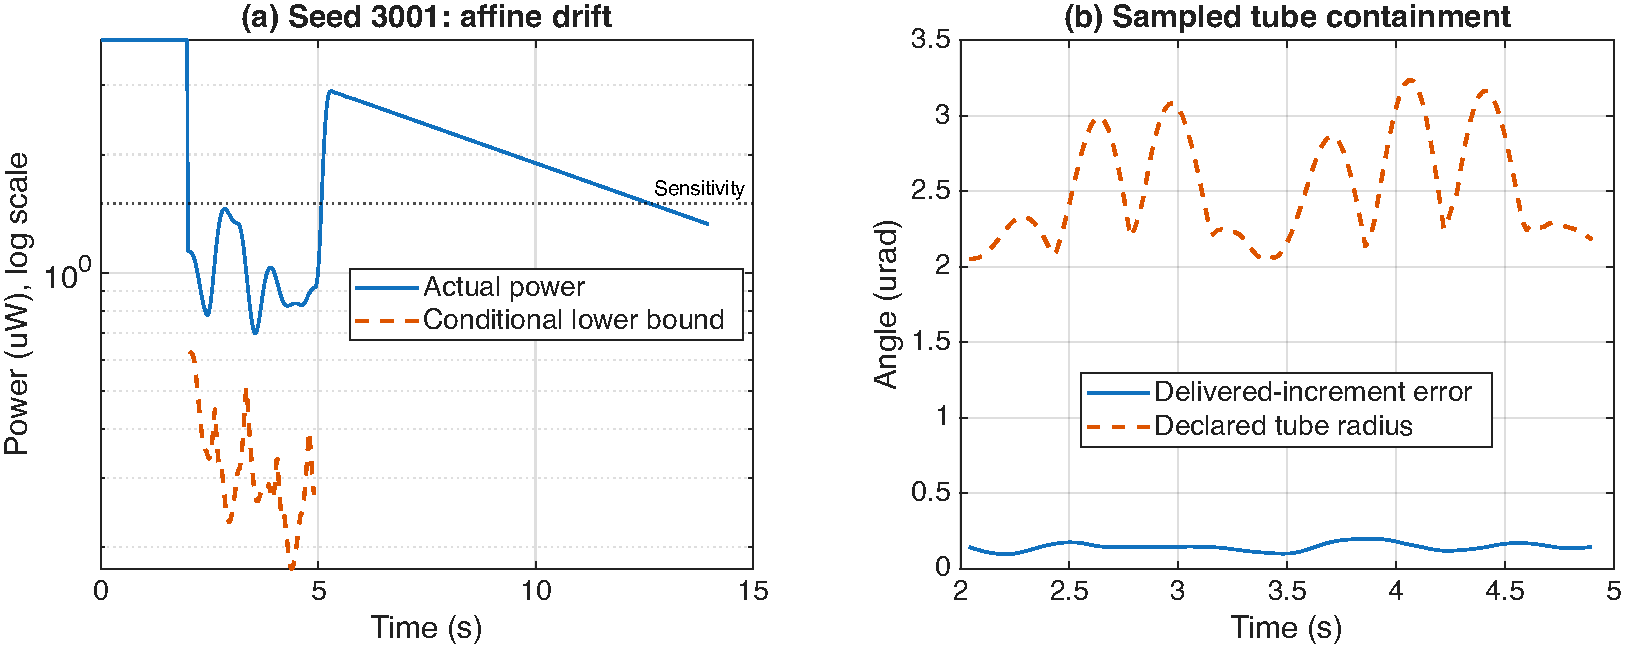
\includegraphics[width=\textwidth]{certificate_trace.pdf}
\caption{First primary seed (3001), selected in advance for representative trace reporting. The lower power curve applies only during the probe and is conservative. Delivered-increment error stays inside the declared finite-model tube. The plot does not establish continuous-time or post-probe safety.}
\label{fig:certificate}
\end{figure*}

\section{Selection and Diagnosis Algorithm}
The candidate library has the balanced rows $[+x,-x,-x,+x,+y,-y,-y,+y]$, amplitudes $\{2,4,6,8\}\um$, and dwell times $\{0.36,0.50\}$~s. The rows have zero constant and linear temporal moments in the quasi-static equal-dwell limit. Their two-axis information is isotropic and reaches the elementary bound $\lambda_{\min}(Q^TPQ)\leq\norm Q_F^2/2$ when no energy is lost to projection. Actual dynamic information is calculated from predicted settled motion, not inferred from that equality.

The first-order predicted statistical radius must be below $1\um$. This is a feasibility heuristic, not a robust lower information guarantee for every uncertain trajectory. The delivered-motion tube is used for service certification, while actual measured rank and fit uncertainty are checked after the probe. A safe-to-attempt probe can still fail to diagnose.

Among feasible candidates, minimize
\begin{equation}
 J_p=T_p+0.03\,\mu\mathrm{rad}^{-2} E_p,\quad
 E_p=\Delta t\sum_i\norm{\bar q_i}^2.
\end{equation}
Here $T_p$ is seconds and $E_p$ is expressed in $\mu$rad$^2$~s, so the score has units seconds. This is a weighted tradeoff, not lexicographic duration minimization or an electrical-energy objective. Search is exact over the library only.

\begin{table}[t]
\caption{Uncertainty-aware diagnosis procedure (UAD).}
\small
\begin{minipage}{\columnwidth}
\begin{enumerate}
\item Observe encoder angle and power. Apply the common three-sample residual trigger after warmup; no injection schedule enters the decision.
\item Refuse darkness. Construct the simultaneous power interval. Enable acquisition only if its upper endpoint is below sensitivity; otherwise retain the working-link budget.
\item Enclose current optical error. For each clamp-valid candidate, evaluate predicted information, the delivered-increment tube, and the lower-power outage count.
\item Select the minimum-score feasible candidate. If none exists, record abstention without diagnosis credit.
\item Execute a causal held reference, retain the last 40\% of each dwell, and fit the measured data using noise-aware GLS.
\item Reject censored, rank-deficient, imprecise or inconsistent fits. Correct pointing only after an accepted significant offset and a sufficient estimated lower aligned-power margin.
\end{enumerate}
\end{minipage}
\label{tab:algorithm}
\end{table}

The prior DAP method instead compares a point-valued current power with sensitivity, uses a nominal zero-start trajectory, and fits a constant-variance affine projection. Ablations remove the proposed tube or restore the point gate. An additional fixed-probe GLS comparator separates estimator effects from selection. The linear parameter filter applies Kalman updates \cite{kalman} to the transformed observation; the ES comparator does not claim a certified fault diagnosis.

For $K$ candidates of $H$ samples, online certificate/search time and stored trajectories are $O(KH)$. The offline finite-model enclosure costs $O(KMN)$ small-matrix operations for $M$ models. With $p\leq5$ regression coefficients and $I_f$ iterations, GLS takes $O(I_fNp^2+p^3)$ time and $O(Np)$ workspace. These operation counts are separate from the plant simulation.

\begin{figure*}[t]
\centering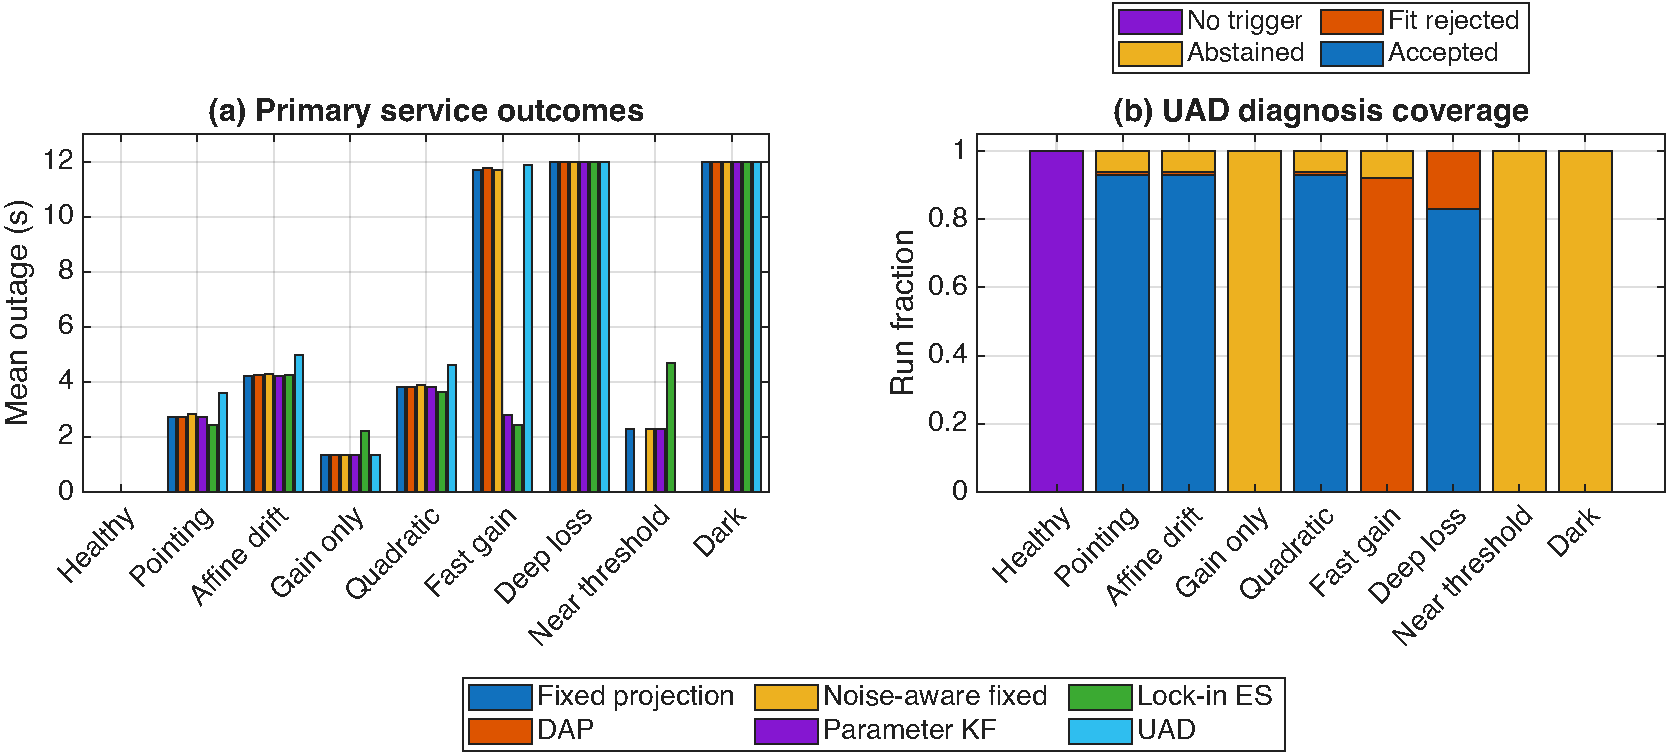
\includegraphics[width=\textwidth]{primary_comparison.pdf}
\caption{Primary service outcomes and the proposed selector's diagnosis coverage. ES uses a larger excitation-time budget and is not credited with a fault diagnosis. Refusal and fit rejection remain visible; they are not counted as successful recovery. All cases, including unfavorable ones, are retained.}
\label{fig:primary}
\end{figure*}

\section{Experimental Design and Verification}
\subsection{Preservation, reproduction, and final protocol}
Before method changes, SHA-256 hashes recorded the original implementation and artifacts. All 5,400 prior primary and 3,600 prior sensitivity trials were rerun; every saved scalar metric matched. Outage and angular excitation were independently recalculated from regenerated traces. Saved binary tables and 54 retained representative traces were also checked, and four saved Simulink metric sets reconstructed. These are same-kernel reproductions, not independent physical replications.

The new frozen protocol uses 100 untouched primary seeds, 3001--3100, for nine scenarios and 12 methods: \NPrimary\ runs. The scenarios are healthy, fixed pointing error, pointing with affine log-gain decline, decline without pointing error, quadratic decline, fast varying gain, deep attenuation, near-threshold gain, and darkness. Pointing magnitude is $(20+6\cos s)\um$ with direction $0.4+0.9\sin s$ radians for seed $s$. Faults begin at 2~s and persist; the decision receives neither onset nor label.

Affine gain is $\exp[-0.09(t-2)]$, quadratic gain is $\exp[-0.008(t-2)^2]$, and fast gain is $\exp[-0.045(t-2)+0.16\sin(4(t-2))]$ after onset. Deep attenuation uses gain 0.18 and near-threshold operation 0.41. These are declared disturbances, not measured spacecraft statistics. All methods share exogenous sample-indexed disturbances within a configuration.

The six original comparator classes remain available. Fixed diagnostic probes use eight $6\um$, 0.36-s dwells. Historical DAP retains its original 0.35/0.50-s library in the common causal wrapper; new results are not substituted for its historical values. Every diagnosis method gets one attempt and the same trigger. ES is allowed eight seconds of post-trigger excitation, a larger budget disclosed when comparing service. Its zero acceptance count means it is a tracker, not that a completed diagnostic fit was rejected.

Development seeds were disjoint. ES gain was selected from $\{0.1,0.3,0.6\}$ and parameter-filter process variance from $\{0,10^{-4},10^{-2}\}$ across all nine development scenarios and noise levels one/five. The selected values are 0.3 and zero, respectively. A poorly conditioned nonlinear EKF development attempt was retained in the evidence but not used as a weakened final comparator; the transformed linear filter avoids that representation problem. Final evaluation outcomes did not select the method or baseline settings.

\begin{figure*}[t]
\centering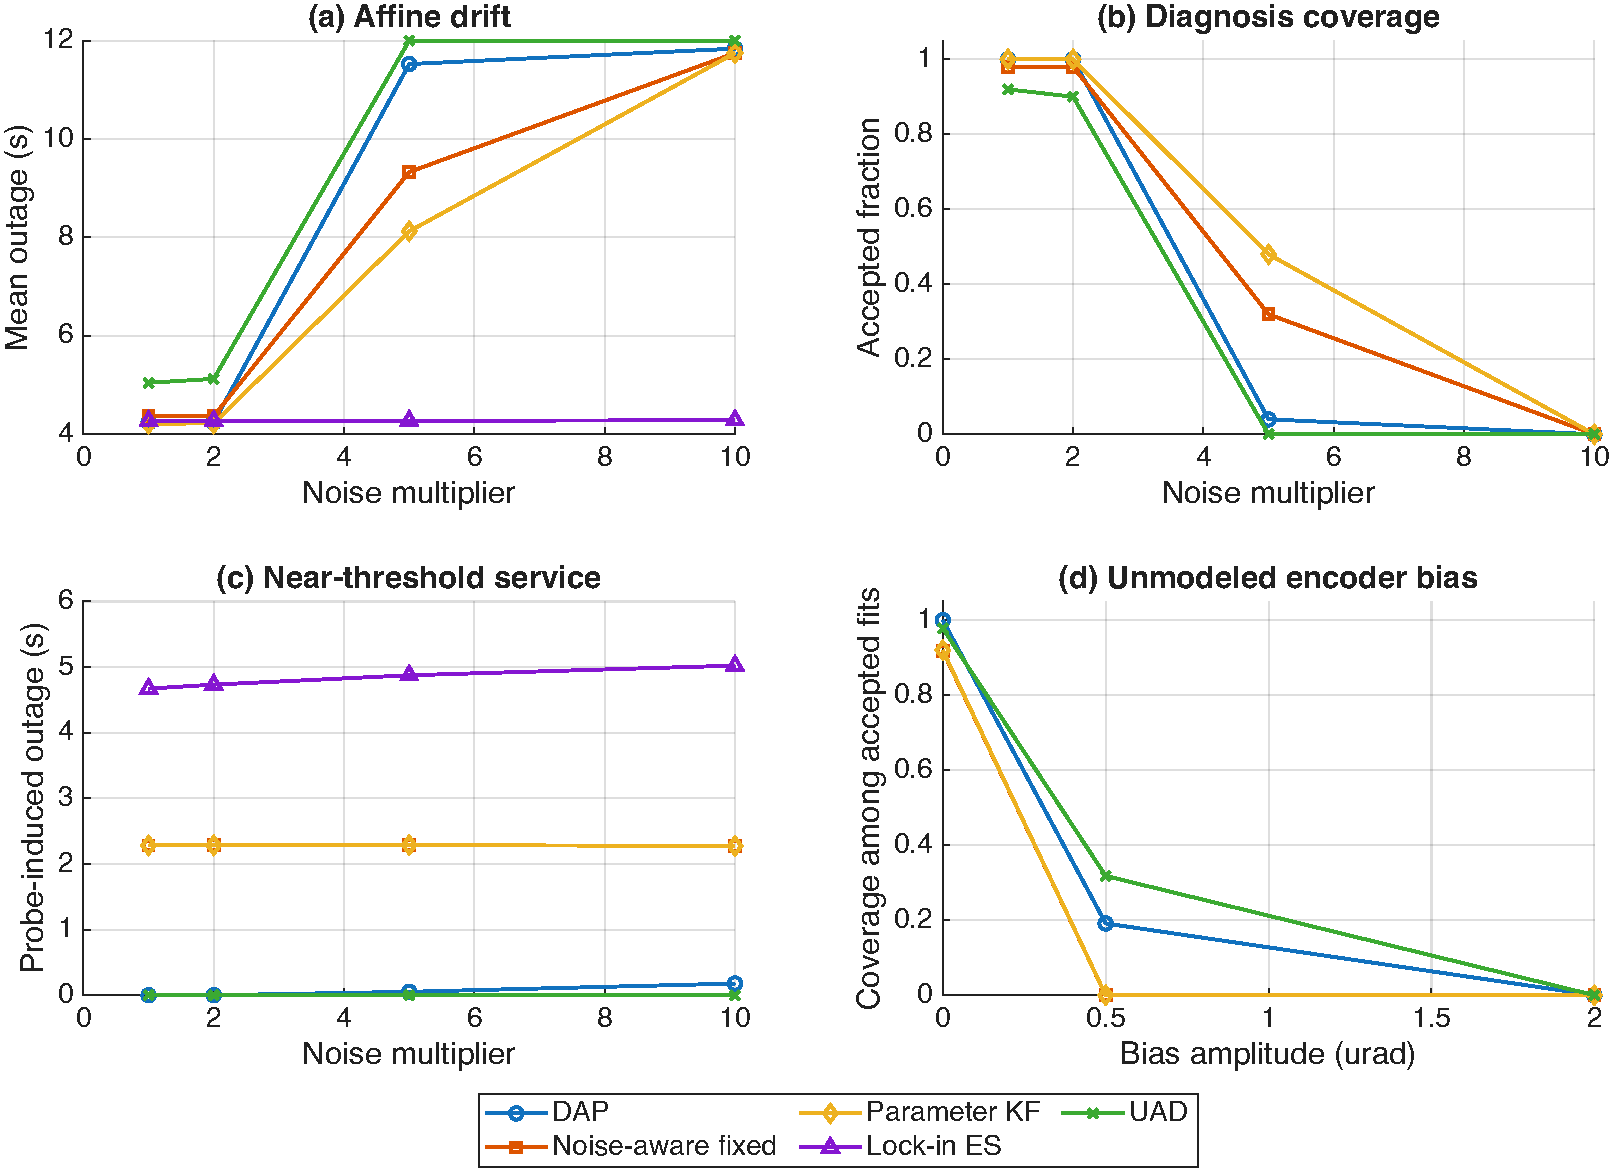
\includegraphics[width=\textwidth]{sensitivity.pdf}
\caption{Sensitivity to noise and unmodeled bias. Approximate covariance can be misleading: accepted-fit coverage collapses under encoder bias. UAD's zero near-threshold outage is accompanied by diagnostic abstention; its large-noise recovery is worse than the tracker and parameter-filter alternatives.}
\label{fig:sensitivity}
\end{figure*}

\subsection{Sensitivity, metrics, and statistics}
An additional \NSensitivity\ runs use 50 new seeds, 4001--4050, in prespecified sweeps of noise, gain slope, curvature, fast variation, divergence, offset magnitude, actuator parameters, encoder bias, link margin, library size, confidence level, outage budget, and sample step. Some conditions deliberately violate declared sets or gain assumptions. They are reported as out-of-model tests. The complete sweep and method list is supplied with machine-readable protocol files.

Outage is integrated over $[2,14)$~s; final availability uses the last two seconds. Each run records accepted and all finite-fit errors, rejection, abstention, missed diagnosis, false correction, mean/median/upper-tail outage summaries, probe count/time, angular excitation, accepted-diagnosis time, confidence coverage, and certificate/tube/budget violations. No estimate yields an undefined error. Abstention is not diagnosis, and zero outage on an initially usable link is not recovery.

A passive counterfactual shares the same exogenous inputs. Probe-induced outage counts sampled times when the active method is down and passive is up; this is a simulator-defined potential outcome, not hardware causal evidence. Angular excitation is not total electrical energy. Online wall time and retained numerical buffer size are measured; they are not worst-case embedded execution time or total process peak memory.

The statistical unit is the run seed. Main UAD--DAP outage differences use 5,000 paired bootstrap resamples, descriptive 95\% intervals, and approximate Bonferroni-adjusted percentile limits for the nine-scenario family. Time samples are not independent replicates. Sensitivity results are exploratory. Zero events among about 100 selected runs cannot establish a one-percent field risk; the zero-event one-sided identical-Bernoulli reference upper bound is approximately 3\%, with additional population assumptions needed for that interpretation.

\subsection{Model and record checks}
MATLAB R2026a Update~3 executes the held-input RK4 model. Independent algebraic tests verify the sharp angular bound, measurement envelope, discrete predictor, exact affine invariance, rank rejection, covariance scaling, mismatch counterexample, candidate score, deterministic execution, darkness, healthy operation, and insufficient-power correction refusal. Numerical disk-aperture quadrature differs from the source small-aperture optical approximation by at most $1.758\times10^{-4}$ relative error over the tested 0--$60\um$ range. This validates an approximation within the Gaussian model, not the hardware model. Full spacecraft pointing requires additional stages and budgets \cite{baeck}; hardware reviews and mission summaries do not calibrate this terminal \cite{actuators,nasa}.

All \NTotal\ new metric rows were checked against saved per-run scientific traces. Passive masks were regenerated and saved for sensitivity counterfactual reconstruction. The first evaluator export omitted the requirement that the offset remain constant throughout a probe; \PremiseFlagRepairs\ affected premise labels were corrected explicitly without deleting bound failures or altering decisions. Exact frozen source and raw exports are retained. The evaluator-only repair was regression-tested and the affected cases reexecuted against corrected records. This distinction is necessary because early probing can overlap a later injected fault.

\begin{table*}[t]
\caption{Primary comparison: 100 seeds per row. Error is the median conditional on an accepted diagnosis; the acceptance denominator is shown. All finite-fit errors, abstentions, additional baselines and complete sensitivity records are supplied separately. Energy is angular excitation, not electrical consumption.}
\centering\small
\begin{tabular}{llrrrrr}\toprule
Scenario & Method & Accepted & Accepted error ($\mu$rad) & Mean outage (s) & P95 outage (s) & Energy ($\mu$rad$^2$ s)\\\midrule
\PrimaryRows
\bottomrule\end{tabular}
\label{tab:results}
\end{table*}







\section{Results}
\subsection{Certificate verification and diagnostic cost}
Complete UAD selects \SelectedCertificates\ primary probes. Of these, \ValidCertificates\ satisfy the checked optical, finite-model and measurement-event premises; \ValidViolations\ observed lower-bound violations occur in that subset. Figure~\ref{fig:certificate} illustrates how conservative the enclosure can be. This is conditional verification, not an empirical demonstration of a universal one-percent risk target.

The additional conservatism has a measurable cost. With affine attenuation drift, UAD accepts \UADDriftAccepted/100 diagnoses and has mean outage \UADDriftOutage~s, compared with \DAPDriftAccepted/100 and \DAPDriftOutage~s for DAP. The paired mean difference is $+\DriftDifference$~s, with descriptive 95\% interval $[\DriftCILow,\DriftCIHigh]$~s. Sequential projection and the parameter filter reach \FixedDriftOutage~s and \KFDriftOutage~s, respectively. Thus the proposed selector does not improve recovery speed in this condition.

For constant pointing error, UAD outage is \UADPointingOutage~s versus \DAPPointingOutage~s for DAP and \ESPointingOutage~s for ES. Its primary refusals and upper-percentile outage are visible in Table~\ref{tab:results}; a small accepted-fit error must not hide those missed diagnoses. UAD uses \UADDriftEnergy~$\mu$rad$^2$~s mean angular excitation in the affine-drift case, versus \DAPDriftEnergy\ for DAP, but lower excitation alone is not evidence of lower total energy or greater operational benefit.

\subsection{Near-threshold operation and noise}
At nominal noise, both DAP and UAD preserve the near-threshold link by refusing diagnosis, while fixed probing causes outage. Under fivefold noise, the sensitivity set gives DAP \DAPNoiseFalseAcq\ false acquisition enablements in 50 runs and mean outage \DAPNoiseNearOutage~s. UAD has \UADNoiseFalseAcq\ such events and \UADNoiseNearOutage~s outage, with no accepted diagnosis. The simultaneous gate is theoretically responsible for the conditional mode-error result, but the full high-noise comparison also includes candidate and tube feasibility. It cannot attribute every empirical difference solely to the gate.

High-noise diagnosis remains weak. At fivefold noise with affine decline, noise-aware fixed probing accepts \GLSNoisyDriftAccepted/50 fits and has outage \GLSNoisyDriftOutage~s; the parameter filter accepts \KFNoisyDriftAccepted/50 with \KFNoisyDriftOutage~s. UAD accepts \UADNoisyDriftAccepted/50 and has \UADNoisyDriftOutage~s outage, whereas ES achieves \ESNoisyDriftOutage~s without a certified fault diagnosis. Some candidate probes fail the declared enclosure/information requirements. Those refusals are retained rather than relaxed to improve a preferred metric.

\subsection{Fast gain, deep loss, and biased sensing}
Fast variation distinguishes estimator failure from physical irrecoverability. DAP and UAD have outages \DAPFadingOutage~s and \UADFadingOutage~s and no accepted fits. The parameter filter reaches \KFFadingOutage~s and ES \ESFadingOutage~s. Therefore the earlier affine-fit failure cannot be generalized to all optical recovery methods. The tracker uses more excitation time and produces no accepted fault label, while the parameter filter's approximate confidence must be read alongside coverage measurements.

Deep attenuation remains physically irrecoverable: $0.18p_0\simeq0.703~\mu$W is below sensitivity at perfect alignment. No method restores service by pointing. Healthy runs produce no unnecessary diagnostic probe; darkness remains uncertain rather than a uniquely identified blockage.

At a $[2,-1]\um$ unmodeled encoder bias, accepted-fit coverage collapses for the tested estimators, including \UADBiasDriftCoverage\% for UAD. Bias shifts the angle reference and is observationally confounded with offset in this measurement model. A small residual or nominal radius does not repair that structural problem. The source's independent rate/torque channels would require a separately analyzed bias-observer integration; they are not silently supplied to the optical estimator.

\subsection{Mid-probe faults and model limitations}
In the 0.9-divergence sweep, the altered aligned power can trigger diagnosis before the scheduled fault, despite being inside the declared divergence range. The fault then changes $b$ during the probe. UAD has \UADBeamEarlyBoundFailures/50 observed bound failures for the pointing case and mean outage \UADBeamEarlyOutage~s; no such run meets the constant-offset premise. These are genuine operational failures outside the certificate's hypotheses, not successful service preservation and not counterexamples to a static-offset theorem. They expose a limitation of a nominal residual trigger combined with an unpredictable future fault.

The sensitivity record contains \SensitivityUADBoundFailures\ total UAD bound failures across all tested configurations; none is removed from the raw data. Conditions with bias, parameters outside the finite set, excessive gain decline or mid-probe offset changes must be distinguished from in-premise checks. The additional sensor-envelope and actuator assumptions make the certificate more defensible than a nominal surrogate, but also restrict its applicability.

For the specified in-set actuator mismatch, UAD affine-drift outage is \UADMismatchDriftOutage~s compared with \DAPMismatchDriftOutage~s for DAP. The method does not become generally robust merely because this finite case is enclosed. A real actuator estimated between grid points has no certificate from this six-member construction.

\section{Discussion and Scope}
The study supports a conditional optical-power analysis, a corrected acquisition-mode decision, and quantified diagnostic costs. It does not support a claim of universally better recovery. Stronger architecture baselines can recover conditions where the proposed affine fit abstains or fails. The comparison therefore separates safe-to-attempt excitation, successful diagnosis, pointing recovery, and service preservation.

The centered-ball angular inequality is exact over the stated uncertainty balls, while the sensor event and finite-model impulse enclosure provide explicit conditions for a sampled certificate. These statements are narrower than a flight safety guarantee. Actual tails may be non-Gaussian, actuator parameters may not belong to a finite set, divergence/gain bounds may be inaccurate, and faults can evolve during probing. A certificate checker must expose these assumptions rather than report an unqualified ``safe'' flag.

Physical parameters remain assumptions. The numerical aperture check and discrete predictor verification are independent calculations of the same model, not optical-bench or hardware-in-the-loop validation. No field measurements, calibrated receiver curve, thermal gain law or actuator uncertainty identification are available. A complete spacecraft link additionally requires receiver pointing, geometry, acquisition, attitude coupling, queues and network routing. Existing four-satellite Simulink runs replace only the optical estimator; their slight steady-gain performance penalty is not validation of the full UAD selector.

The baseline implementations are disclosed and executable, but published complete optical systems and the general constrained-AFD methods were not faithfully reproduced. This limits state-of-the-art conclusions. The exact relationship to recent link-margin-aware acquisition and related patent literature also merits further specialist assessment. A system-specific derived certificate should not be presented as the invention of safe active diagnosis.

\balance
\section{Conclusion}
Expressing Gaussian received power relative to the current optical condition yields a bound in delivered angular increment without assuming zero initial angle. The centered-ball angular loss is sharp, and a simultaneous sensor event supports acquisition gating at an adaptively selected start. With a verified finite-model sampled-actuator tube, the result bounds sampled probe-window outage under explicit optical and measurement hypotheses.

Executed experiments show the price of that statement: increased abstention and outage in several recoverable cases, no high-noise diagnosis advantage, and useful service preservation near sensitivity. Parameter filtering and extremum seeking recover some fast-gain cases rejected by the affine fit. Bias, mid-probe faults and model-set violations remain consequential failures. The contribution is a reproducible conditional analysis and tradeoff study, with physical validation and broader baseline reproduction still required.

\section*{Data, Code, and Assistance Disclosure}
Supplementary files include the preserved original benchmark, frozen V4 configurations and sources, full per-run scientific traces, original and explicitly corrected premise labels, aggregate tables, plotting/analysis scripts, regression tests, and audit records. Code reuse is attributed to the source project \cite{source}; the new implementation does not imply authorship of its original terminal model.

OpenAI Codex assisted the mathematical formulation, literature investigation, implementation, analysis, tests, figures, and drafting of all manuscript sections. Numerical results were generated by the recorded MATLAB executions. This disclosure describes substantive assistance in accordance with IEEE guidance \cite{aipolicy}; it does not represent independent human verification or assign authorship to an AI system.

\begin{thebibliography}{99}
\bibitem{guelman} M. Guelman \emph{et al.}, ``Acquisition and pointing control for inter-satellite laser communications,'' \emph{IEEE Transactions on Aerospace and Electronic Systems}, vol. 40, no. 4, pp. 1239--1248, 2004, doi: \href{https://doi.org/10.1109/TAES.2004.1386877}{\nolinkurl{10.1109/TAES.2004.1386877}}.
\bibitem{cai} W. Cai, A. N. Alhashim, I. N’Doye, T. M. Laleg-Kirati, ``An Extremum Seeking Control Based Approach for Alignment Problem of Mobile Optical Communication Systems,'' \emph{IFAC-PapersOnLine}, vol. 53, no. 2, pp. 5368--5374, 2020, doi: \href{https://doi.org/10.1016/j.ifacol.2020.12.1519}{\nolinkurl{10.1016/j.ifacol.2020.12.1519}}.
\bibitem{mai} V. Mai, H. Kim, ``Beaconless angle-of-arrival tracking with improved receiver sensitivity and tracking precision for free-space optical communications,'' \emph{Optics Communications}, vol. 527, Art. no. 128963, 2023, doi: \href{https://doi.org/10.1016/j.optcom.2022.128963}{\nolinkurl{10.1016/j.optcom.2022.128963}}.
\bibitem{cheong} S. Cheong, I. R. Manchester, ``Input design for model discrimination and fault detection via convex relaxation,'' \emph{2014 American Control Conference}, pp. 684--690, 2014, doi: \href{https://doi.org/10.1109/ACC.2014.6859400}{\nolinkurl{10.1109/ACC.2014.6859400}}.
\bibitem{palmer} K. A. Palmer, G. M. Bollas, ``Active fault diagnosis for uncertain systems using optimal test designs and detection through classification,'' \emph{ISA Transactions}, vol. 93, pp. 354--369, 2019, doi: \href{https://doi.org/10.1016/j.isatra.2019.02.034}{\nolinkurl{10.1016/j.isatra.2019.02.034}}.
\bibitem{guo} Y. Guo, Q. Liu, Z. Wang, Z. Zhang \emph{et al.}, ``Active fault diagnosis for linear stochastic systems subject to chance constraints,'' \emph{Automatica}, vol. 156, Art. no. 111194, 2023, doi: \href{https://doi.org/10.1016/j.automatica.2023.111194}{\nolinkurl{10.1016/j.automatica.2023.111194}}.
\bibitem{massa} N. Massa, J. A. Paulson, ``Optimal input design for guaranteed fault diagnosis of nonlinear systems: An active deep learning approach,'' \emph{Control Engineering Practice}, vol. 153, Art. no. 106118, 2024, doi: \href{https://doi.org/10.1016/j.conengprac.2024.106118}{\nolinkurl{10.1016/j.conengprac.2024.106118}}.
\bibitem{safees} A. Williams, M. Krstic, A. Scheinker, ``Semiglobal Safety-Filtered Extremum Seeking With Unknown CBFs,'' \emph{IEEE Transactions on Automatic Control}, vol. 70, no. 3, pp. 1698--1713, 2025, doi: \href{https://doi.org/10.1109/TAC.2024.3469785}{\nolinkurl{10.1109/TAC.2024.3469785}}.
\bibitem{yan} K. Yan, B. Guo, Y. Zhou, X. Xue \emph{et al.}, ``Link-Margin-Aware joint parameter optimization for scanning and acquisition of optical inter-satellite link,'' \emph{Optics Communications}, vol. 616, Art. no. 133342, 2026, doi: \href{https://doi.org/10.1016/j.optcom.2026.133342}{\nolinkurl{10.1016/j.optcom.2026.133342}}.
\bibitem{es} M. Krstić, H. Wang, ``Stability of extremum seeking feedback for general nonlinear dynamic systems,'' \emph{Automatica}, vol. 36, no. 4, pp. 595--601, 2000, doi: \href{https://doi.org/10.1016/S0005-1098(99)00183-1}{\nolinkurl{10.1016/S0005-1098(99)00183-1}}.
\bibitem{cao} F. Cao, F. Jia, X. He, ``Input Design for Active Fault Detection: Reconciling System Control Objectives,'' \emph{IEEE Transactions on Cybernetics}, vol. 54, no. 7, pp. 3931--3942, 2024, doi: \href{https://doi.org/10.1109/TCYB.2023.3331971}{\nolinkurl{10.1109/TCYB.2023.3331971}}.
\bibitem{source} Satellite-Optical-Fault-Recovery, source terminal model and V2 implementation, local archived snapshot \texttt{0bc453ffa0ad}. \href{https://github.com/kaushalrog/Satellite-Optical-Fault-Recovery}{Source repository}; accessed Oct. 23, 2026.
\bibitem{kalman} R. E. Kalman, ``A New Approach to Linear Filtering and Prediction Problems,'' \emph{Journal of Basic Engineering}, vol. 82, no. 1, pp. 35--45, 1960, doi: \href{https://doi.org/10.1115/1.3662552}{\nolinkurl{10.1115/1.3662552}}.
\bibitem{baeck} K. Baeck, J. Wi, H. Yoon, ``Analytic pointing error evaluation on nano-satellite laser communication system,'' \emph{Optics Communications}, vol. 559, Art. no. 130419, 2024, doi: \href{https://doi.org/10.1016/j.optcom.2024.130419}{\nolinkurl{10.1016/j.optcom.2024.130419}}.
\bibitem{actuators} M. Milaševičius, L. Mačiulis, ``A Review of Mechanical Fine-Pointing Actuators for Free-Space Optical Communication,'' \emph{Aerospace}, vol. 11, no. 1, Art. no. 5, 2024, doi: \href{https://doi.org/10.3390/aerospace11010005}{\nolinkurl{10.3390/aerospace11010005}}.
\bibitem{nasa} NASA Small Spacecraft Systems Virtual Institute, ``State-of-the-art small spacecraft technology: Communications.'' \href{https://www.nasa.gov/smallsat-institute/sst-soa/soa-communications/}{NASA communications overview}; accessed Oct. 23, 2026.
\bibitem{aipolicy} IEEE Author Center, ``Submission and peer review policies: Use of AI by authors.'' \href{https://journals.ieeeauthorcenter.ieee.org/become-an-ieee-journal-author/publishing-ethics/guidelines-and-policies/submission-and-peer-review-policies/}{IEEE policy}; accessed Oct. 23, 2026.
\end{thebibliography}

\end{document}
